Showing PES:
 - benzene
 - near-threshold PES
 - Find systems where PES is known for different photon energies

There is a paper\cite{vibPES} with vibronically resolved PES from experiment.\\
PES of N2 with 'angular resolution' (latter not directly) \cite{PESN2}.

purine and pyrimidine: comparison to Green's function methods via the \cite{PottsHolland}-paper.

For AlO$^-$ there is a paper with 2 spectra with one and two transitions each, having vibrational
structure\cite{AlO}.

Atomic Systems have some experimental data as well: For Xe and Kr the spectra at photon energies of 150$\,$eV are shown in reference \cite{KrXe}.

A combined theoretical and experimental study on CH$_2$F$_2$ is in ref. \cite{ch2f2}. Here, theory is quite bad and experiment is also angular resolved, thus may be interesting.

\section{Benchmarks and Tests on the Formalism}
\label{ch:resBench}

\subsection{Comparison of Formulations}
While the unconjugated Burnett-formulation was not very successfull, the conjugated formulations of Burnett and Astley-Leis might both be interesting to compare for a quantum mechanical problem.
Since the conjugated Burnett elements lead to infinitely large matrix elements, here the Astley-Leis elements (\ref{eq:ALelem}) will be compared with a symmetrised form where the shape functions are of the form
\begin{equation} 
 \Phi(\vec{r}) = \sqrt{D(r)}\varphi(\vec{r}) e^{-ik\mu(r)}
\end{equation}
for both, the test- and ansatz functions.
Using this formulation, only the kinetic energy expression changes to
\begin{multline}
\int \left(\nabla \Phi_i(\vec{r})\right)\left(\nabla \Psi_j(\vec{r})\right) d\vec{r}
=\int \frac 14 \frac{D'(\vec{r})D'(\vec{r})}{D(\vec{r})} \varphi_i(\vec{r})\varphi_j(\vec{r})
+ \frac 12 D'(\vec{r}) \left( \varphi_i(\vec{r})\varphi_j'(\vec{r}) +\varphi_i'(\vec{r})\varphi_j(\vec{r})\right) \\
+ D \left( \varphi_i'(\vec{r})\varphi_j'(\vec{r})+ik\mu'(r) (\varphi_i(\vec{r})\varphi_j'(\vec{r}) - \varphi_i'(\vec{r})\varphi_j(\vec{r}))
     - (ik \mu'(r))^2\varphi_i(\vec{r})\varphi_j(\vec{r})\right) d\vec{r}.
\end{multline}
\textcolor{red}{Discussion of spectrum:
\begin{itemize}
   \item What is the meaning of imaginary eigen-values? How to interprete results?
   \item Should one sort the `initial' energies to make it comparable to `symmetrised'?
   \item Which conclusions to draw from this study?
\end{itemize}}
\begin{wrapfigure}{r}{0.5\textwidth}
\includegraphics[width=0.5\textwidth]{Figures/IFem_form_spectra}
\caption{The first 50 eigenvalues obtained with the original Astley-Leis formulation (imaginary part not shown) and with the symmetrised form (\ref{eq:ALsymm}).}
\label{fig:IFEMform_spect}
\end{wrapfigure}
\textcolor{blue}{Discussion of Spherical Waves:
\begin{itemize}
   \item In both cases: very strong mixing of quantum numbers
   \item Is the difference in nature more different than that obtained from slightly
         differing parameters?
   \item The symmetrised form indeed seems to damp the $s$- and $p$-waves out.
   \item Can one understand these expansions/differences in terms of damping for large $r$?
   \item Which conclusions can be drawn from this study?
\end{itemize}}
\begin{figure}
\begin{subfigure}{0.5\textwidth}
\includegraphics[width=\textwidth]{Figures/Ifem_form_init}
\end{subfigure}
\begin{subfigure}{0.5\textwidth}
\includegraphics[width=\textwidth]{Figures/Ifem_form_symm}
\end{subfigure}
\caption{Decomposition of the first 31 solutions into spherical waves with anular momenta up to $l=7$.
Left: Astley-Leis-formulation, right: symmetrised form.}
\label{fig:IFEMform_project}
\end{figure}

Investigation of the spectrum as a function of the power $p$ for the symmetric and non-symmetric formulation of the Hamiltonian.
\begin{figure}
\caption{Figure to be placed}
\end{figure}

\subsection{Numerical Convergence}
Tested on Lithium with a sphere with $r_\text{max}=2.8$
1:  Using the mapping of Son with a naive approach, setting the number of circles by hand and growing quadratically with the size  ($N_\text{circle}=20$, $l= 2.0$ , $N= 10$)
2: using the Son scheme with N according to above formula
3: using the tm scheme as described above, p=1
4: using the tm scheme as described above, p=2

\begin{tabular}{|c|c|c|}
\hline
scheme & \#elements & error in energy [a.u.]\\
\hline
1      & 2370      & 0.496220, 0.520199, 0.572279 \\
2      & 2022      & 0.038136, 0.046119, 0.055691 \\
3      & 2166      &-0.003638, 0.027219, 0.050588 \\
4      & 2338      & none converged \\
\hline
\end{tabular}
In these calculations the number of elements were kept as similar as possible.

In the FEM scheme used to compute the FEF, several parameters governing numerical and physical characteristics are used.
The size of the Krylov-subspace does not play a role for the quality of the solution as shown in Figure \ref{fig:E_nev} for the symmetric formulation with a power $p=\frac 12$ of the damping function $D$.
\begin{wrapfigure}{r}{0.5\textwidth}
\includegraphics[width=0.5\textwidth]{Figures/Root_E_nev.pdf}
\caption{The energies of the 20 states that fit the target energy best, depending on the
size of the Krylov-suspace, indicated by the colour.}
\label{fig:E_nev}
\end{wrapfigure}
Such a good behaviour can, however, only be observed for the symmetric case because in case of the non-hermitian formulation the ordering of the eigenvalues can not be done unambiguously.

More important than the subspace used numerically is obviously the size of the sphere used for the FEM description.
\begin{itemize}
   \item `Convergence' speed depends on power of $D$, chose $p=\frac 12$ here.
   \item Increasing box-size leads to contributions of larger $l$ 
   \item Non-symmetric formulation leads to stronger mixing of angular momenta
   \item Spectra converged for $p=1/8$, see Figure \ref{fig:powerSpect} in supplement.
\end{itemize}
\begin{figure}
\includegraphics[width=\textwidth]{Figures/RadWaves_p0_5.pdf}
\caption{The eigen energies for different box sizes (coloured dots in the upper pannel) where the box size is denoted by the colour in atomic units.
The lower pannel shows the decomposition of the solutions into spherical waves for three box sizes, marked by a star in the color bar respecively.}
\label{fig:RadWaves}
\end{figure}

\section{atomic Lithium}
As the smallest system that has multiple electrons in its anionic state as well, Lithium is an important
test object that has theoretical as well as experimental reference data available\cite{Li-R,Li-R1, LiNaRef1}.
Experiment from Moore, cited in \cite{LiNaRef1}; original not found.
Experiment 2 from \cite{LiSonntag}.

\begin{wrapfigure}{l}{0.7\textwidth}
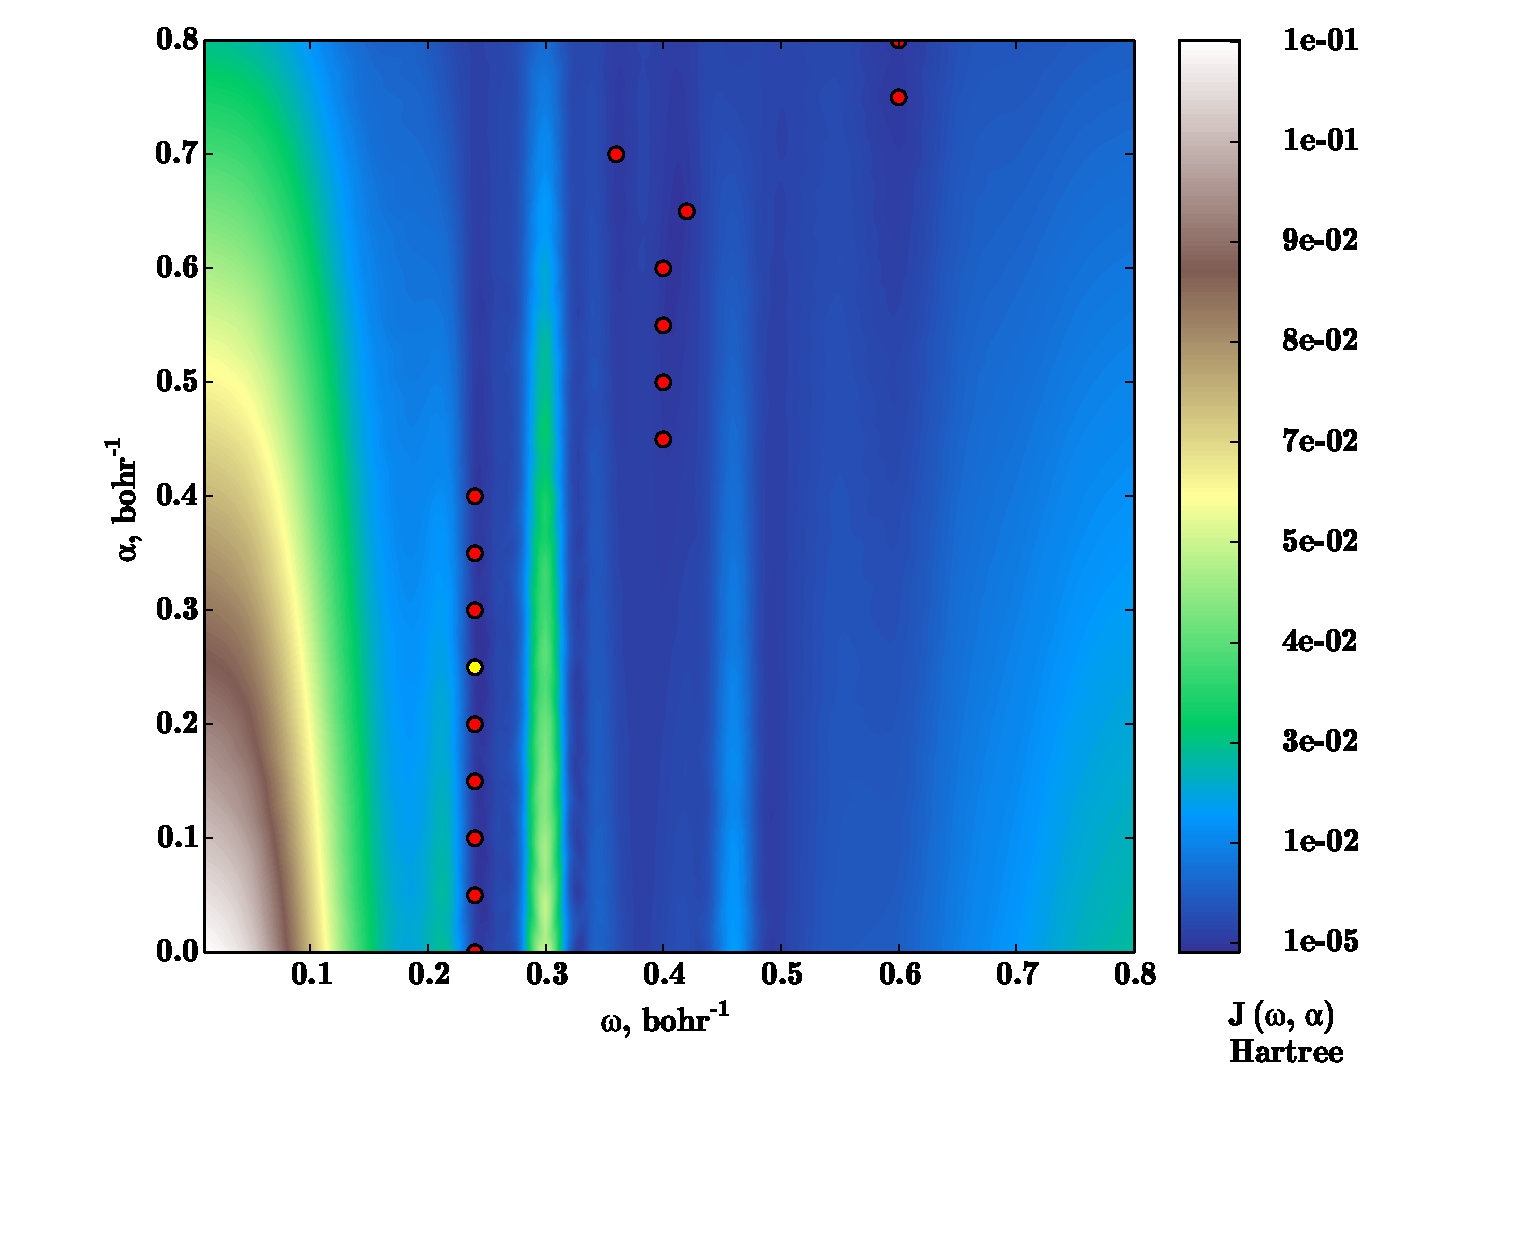
\includegraphics[width=0.69\textwidth]{Figures/Lithium/Lithium_J0_2D_terrain_path_spline_cut}
\caption{The functional $J(\alpha,\omega)$ described in eqation (\ref{eq:J_ao}) for Lithium}
\label{fig:Lith-otrsh}
\end{wrapfigure}

Cross-section: \cite{LiCS}.

The appearance of $2p$-states are accessed by a dipole-transition in the bound part and can not be described within the theory applied here due to the neglect of the conjugate DO term in equation (\ref{eq:fullDO}) \cite{saPonzi}.

\section{Triatomic Linear Molecules}
There are several studies on CO$_2$ \cite{CO2, CO2_highres, HighResLinear, DiffLinear}, CS$_2$ \cite{DiffLinear,HighResLinear}, COS \cite{DiffLinear,HighResLinear} and N$_2$O \cite{DiffLinear}

CS$_2$ is known to have strong correlation effects \cite{2phcederbaum}
\begin{wrapfigure}{l}{0.7\textwidth}
\includegraphics[width=0.69\textwidth]{Figures/CO2_J0_2D_terrain}
\caption{The functional $J(\alpha,\omega)$ described in eqation (\ref{eq:J_ao}) for CO$_2$}
\label{fig:CO2-otrsh}
\end{wrapfigure}

\section{water}
The PES and threshold PES, where the kinetic energy of the photoelectron is kept constant instead of the energy of the photon, of water is experimentally well studied 
for different photon energies.
As example, in Ref. \cite{waterTPE} the PES of water and several TPES of water and heavy water are investigated with high resolution.\\
Similar high accuracy is achieved in Ref. \cite{waterHePES} where the PES of H$_2$O$^+$ and D$_2$O$^+$ are studied with a He1 source, radiating at $537\,$Angs.\\
Further PES are available at higher photon energies:
In \cite{water1200}, photons at energies of $1200\,$eV are used.
A further study of Winter \textit{et. al.} measured spectra at $60$, $75$ $80$, $100$ and $120\,$eV in gas and liquid phase \cite{winterWater}.\\
These studies are of interest here since they yield a variety of different test-cases on a single system that can be used to prove the method being used to be valid.
